\documentclass[tikz,border=10pt]{standalone}
\usepackage{amsmath}
\begin{document}
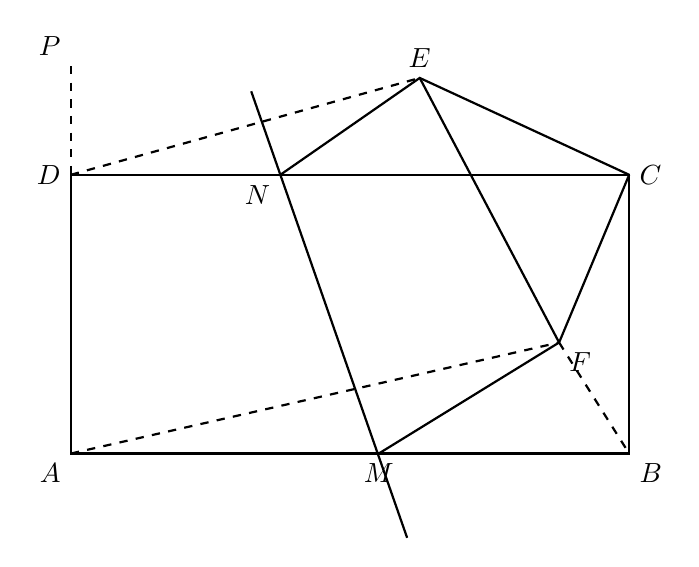
\begin{tikzpicture}[scale=1, line width=0.8pt]

\coordinate (A) at (0,0);
\coordinate (B) at (7.09,0);
\coordinate (C) at (7.09,3.54);
\coordinate (D) at (0,3.54);
\coordinate (P) at (0,4.92);
\coordinate (E) at (4.43,4.77);
\coordinate (N) at (2.66,3.54);
\coordinate (M) at (3.91,0);
\coordinate (F) at (6.20,1.41);
\coordinate (L1) at (2.29,4.60);
\coordinate (L2) at (4.27,-1.07);

\draw (A) -- (B) -- (C) -- (D) -- cycle;

\draw[dashed] (P) -- (D);
\draw[dashed] (D) -- (E);
\draw[dashed] (A) -- (F);
\draw[dashed] (F) -- (B);

\draw (N) -- (E) -- (C);
\draw (C) -- (F) -- (M);
\draw (E) -- (F);
\draw (L1) -- (L2);

\node[above left] at (P) {$P$};
\node[left] at (D) {$D$};
\node[above] at (E) {$E$};
\node[below left] at (N) {$N$};
\node[right] at (C) {$C$};
\node[below right] at (F) {$F$};
\node[below left] at (A) {$A$};
\node[below right] at (B) {$B$};
\node[below] at (M) {$M$};

\end{tikzpicture}
\end{document}
